\documentclass[13pt, a4paper, twoside]{article}
\usepackage[utf8]{inputenc}
\usepackage{geometry}
\usepackage[czech]{babel}
\usepackage{chemformula}
\usepackage{chemfig}
\usepackage{enumitem}
\usepackage{float}
\usepackage{fancyhdr}
\usepackage{caption}
\usepackage{setspace}
\usepackage{multicol}
\geometry{legalpaper, margin=1.05in}
\pagestyle{fancy}
\lhead{\Large Šárka Doležalová, skupina 6}
\rhead{\large 10.12.2020}
\begin{document}
\begin{center}
    \Huge
    Úloha 9: Destilace za sníženého tlaku
\end{center}
\large \onehalfspacing
\section*{Zadané úlohy}
\begin{enumerate}
    \item Vyčistěte předložený ester kyseliny octové destilací za sníženého tlaku.
    \item Sestrojte graf závislosti teploty par na čase.
    \item Zjistěte index lomu produktu.
    \item Zjistěte hustotu produktu.
    \item Na základě změřených vlastností produkt identifikujte.
    
\end{enumerate}
\section*{Teoretický úvod}
\subsection*{Destilace za sníženého tlaku}
Destilace je druh oddělovací metody, kdy se se směs přivádí do bodu varu jedné ze složek a tak se látky oddelují. Snížený tlak je pro destilaci výhodný tím, že můžeme destilovat látky, které by se za normálního tlaku rozkládaly.


Destilaci za sníženého tlaku provádíme v aparatuře, která obsahuje destilační baňku, destilační nástavec, sestupný chladič a alonž. Na alonž se dále zpravidla nasazuje vemínko s malými kulatými baňkami.

\subsection*{Měření indexu lomu}
Index lomu je poměr rychlosti světla ve vakuu a v dané kapalině.
\begin{align*}
    n = \frac{c}{v}
\end{align*}

Index lomu měříme na tzv refraktometru. My užíváme refraktometr Abbeova typu. Jeho jádro se skládá ze dvou hranolů (měřící a osvětlovacího) Mezi ně se vkládá příslušná tekutina. To celé je pozorováno okulárem, abychom zjistili daný index lomu.

\section*{Postup}

\subsection*{Destilace za sníženého tlaku}
Byl navážen 1 g síranu sodného, který byl přidán do neznámého roztoku
96 v 25 ml Erlenmeyerově baňce. Poté byl zazátkován a pečlivě zamíchán.
Vzorek byl přefiltrován přes skládaný filtr do 50 ml kulaté baňky.
Poté byla zvážena 25 ml slzovitá baňka (m=25.62 g).
K destilované směsi bylo přidáno magnetické míchadlo a byla sestavena celá aparatura.
Vpichovaná kolona byla tepelně zaizolováno pomocí vaty a alobalu. Byla zapnuta míchačka a puštěna voda do chladiče.
Dále byla zapnuta membránová pumpa a aparatura byla evakuována zavřením kohoutu pojistné láhve.
Tlak v aparatuře byl ověřen otevřením rtuťového manometru.
Na míchačce byla teplota nejprve nastavena na 50$^\circ$C a poté postupně po 10$^\circ$C zvyšována, aby nedošlo k vykypění směsi.
Teplota lázně byla udržovaná maximálně o 20$^\circ$C vyšší než je byla teplota varu.
Než se teplota ustálila jímáme frakci do 10 ml baňky, po ustálení teploty, byla frakce jímaná do zvážené 25 ml baňky.
Destilace byla ukončena po dodestilování produktu. Baňka s produktem byla zvážena (m=12.77 g) a byl spočítán výtěžek.
Dále byl změřen index lomu produktu, n = 1.398.

\subsection*{Kalibrace automatické pipety}
Automatická pipeta byla kalibrována pomocí destilované vody a analytických vah. Na pipetě byl nastaven objem 1.000 ml. Vody byla pipetována do lékovky, ve které byla zvážena.
Vzorcem $V=\frac{m}{\rho}$ byl spočítán skutečný objem.
Postup byl zopakován pětkrát. A výsledné hodnoty byly zprůměrovány, protože se žádná z nich nelišila o více ne 0,5\%, měření nebylo opakováno. Průměrný hodnota (0.9894 ml), byla poté použita k výpočtu hustoty.

\subsection*{Stanovení hustoty produktu}
Bylo odpipetováno a zváženo 0.9894 ml výsledného produktu. Postup byl proveden pětkrát a hmotnost byla zprůměrována. Vzorcem $\rho= \frac{m}{V}$ byla vypočítána hustota produktu.

\section*{Naměřené hodnoty}

\begin{figure}[H]
    \centering
    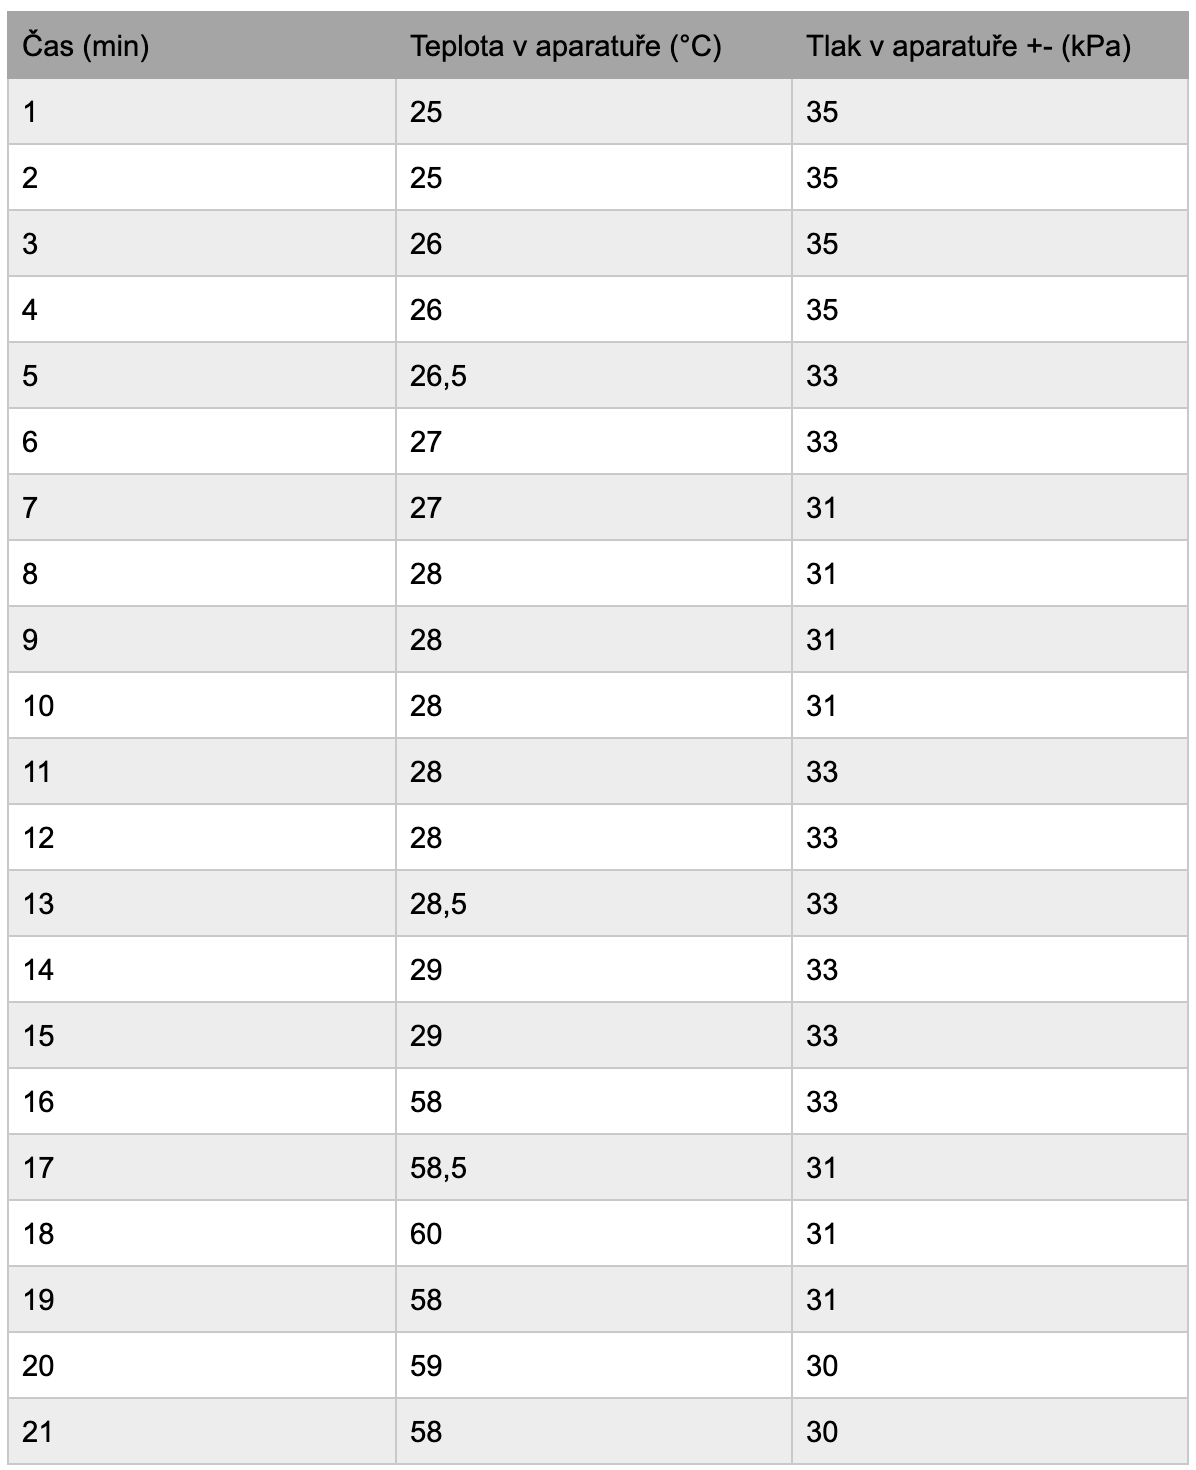
\includegraphics[width=6in]{uloha_9_tab_1.png}
    \caption*{Tab 1. Měření varu za daného tlaku}
\end{figure}


\begin{figure}[H]
    \centering
    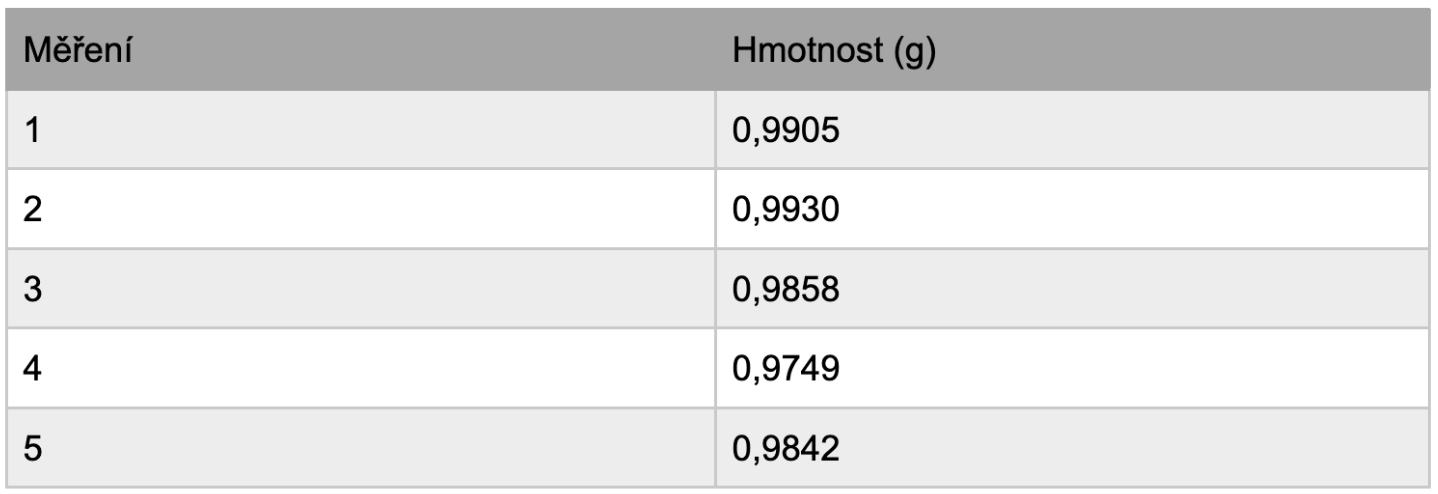
\includegraphics[width=6in]{uloha_9_tab_2.png}
    \caption*{Tab 2. Kalibrace pipety}
\end{figure}



\begin{figure}[H]
    \centering
    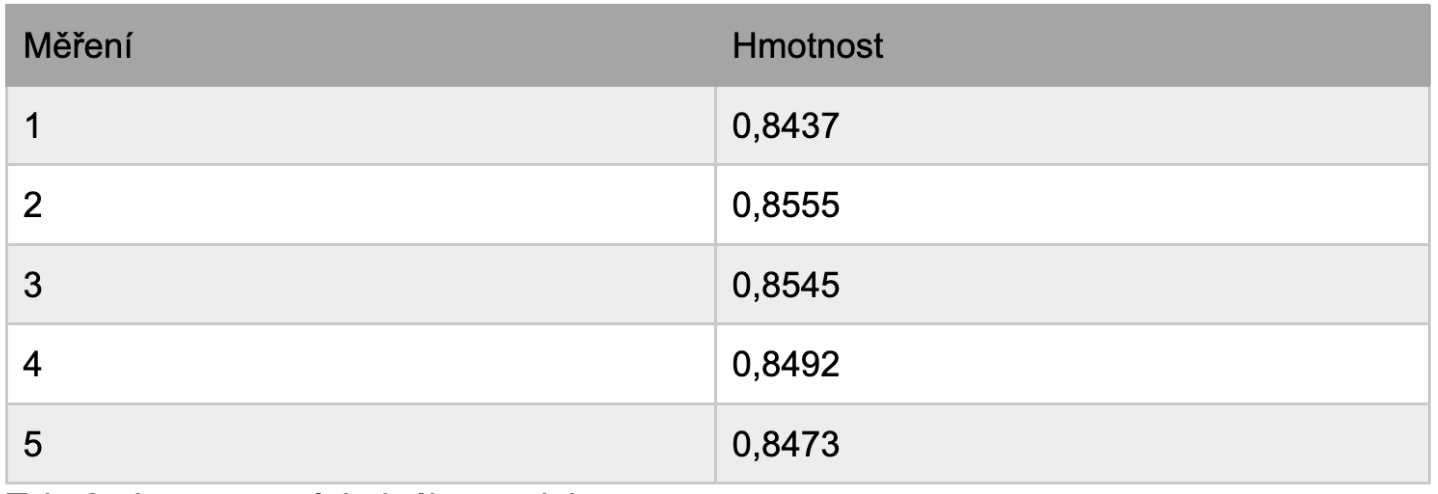
\includegraphics[width=6in]{uloha_9_tab_3.png}
    \caption*{Tab 3. Hmotnost výsledného produktu}
\end{figure}

\section*{Výpočty}
\subsection*{Výtěžek}
\begin{align*}
    V_{produkt} &= \frac{m_{produkt}}{\rho_{produkt}}\\
    V_{produkt} &= 14.86 \: ml
\end{align*}

\begin{align*}
    \alpha &= \frac{V_{produkt}}{V_{nez. vzorek}}\\
    \alpha &= 0.59
\end{align*}

\subsection*{Hustota}
\begin{align*}
    \rho &= \frac{m}{V}\\
    \rho &= 
\end{align*}

\section*{Závěr}
Hodnota indexu lomu (n = 1,398) vycházela mezi butyl-acetátem a pentyl-acetátem a hodnota hustoty ($\rho = 0,85915\: g/cm^3$) vycházela nejblíže hexyl-acetáta. Neznámá látka byla identifikována jako pentyl-acetát. Výtěžek pentyl-acetátu byl $\alpha$= 0,59.



\end{document}